\documentclass{beamer}

\usepackage[utf8]{inputenc}
\usepackage{skak}
\usepackage{listings}
\usepackage{xcolor}
\usepackage{graphicx}

\usepackage[
backend=biber,
style=alphabetic,
citestyle=authortitle-icomp
]{biblatex}

\addbibresource{presentation.bib}

\usetheme{metropolis}

\title{Chesskell: Modelling a Two-Player Game at the Type-Level}
\author{Toby Bailey}
\institute{Department of Computer Science}
\date{\today}

\definecolor{background}{rgb}{0.92, 0.92, 0.92}
\definecolor{comments}{rgb}{0.0, 0.64, 0.0}
\definecolor{keywords}{rgb}{0.0, 0.0, 0.64}
\definecolor{identifiers}{rgb}{0.63, 0.81, 0.94}
\definecolor{strings}{rgb}{1.0, 0.3, 0.0}

\lstset{
    language=haskell,
    basicstyle=\footnotesize\ttfamily,
    backgroundcolor=\color{background},
    keywordstyle=\color{keywords}\bfseries,
    commentstyle=\color{comments}\textit,
    stringstyle=\color{strings},
    % identifierstyle=\color{identifiers},
    breakatwhitespace=true,
    breaklines=true,
    keepspaces=true,
    captionpos=b,
    frame=tlbr,    % Margin at all 4 sides
    framesep=4pt,  % Margin size
    framerule=0pt,
    morekeywords={Eval, Exp, family, instance},
    deletekeywords={map, and, error, take},
    showstringspaces=false
}

% Custom command for all inline code styling
\newcommand{\inline}[1]{\lstinline[basicstyle=\ttfamily]{#1}}

\begin{document}

\frame{\titlepage}

\begin{frame}[standout]

Why do type systems exist?
    
\end{frame}

\begin{frame}{Why do type systems exist?}
Type systems exist because: \pause we want to avoid errors.

(\cite{cardellitypes})

% \pause But not domain-specific logical errors?

% \pause Solution: model your domain in the types!
\end{frame}

\begin{frame}[fragile]{Type Errors}

A type system can prevent certain errors from occurring at all:

\begin{lstlisting}
not 5
\end{lstlisting}

The above will not compile, preventing an error.
    
\end{frame}

\begin{frame}[fragile]{Type Errors cont.}

You have a website, where you sell books.

\pause

For some reason, you use Java to build the server:

\begin{lstlisting}[language=Java]
int noOfPages = -1;
\end{lstlisting}

This is obviously an error. But it compiles!
    
\end{frame}

\begin{frame}[fragile]{Type-Level Programming}

Recent developments to Haskell have focused on performing computation at the type level with \emph{type families} (\cite{opentfs}, \cite{closedtfs}).

Haskell is NOT a dependently typed language; types and values are separated.
    
\end{frame}

\begin{frame}[fragile]{Type Erasure}
In fact, Haskell programs undergo \emph{type erasure}.

\pause

\begin{lstlisting}
x :: Int
x = 3
\end{lstlisting}

Haskell type-level programming involves circumventing type erasure.

\end{frame}

\begin{frame}{Complex Type-Level Computation}

There are other attempts at rule enforcement, in Haskell, at the type level:

\pause

Mezzo - musical composition (\cite{mezzohaskellsymposium})

\pause

BioShake - Bioinformatics workflows (\cite{bioshake})


% Mezzo is an EDSL for musical composition, which can enforce classical harmony rules at the type level (\cite{mezzohaskellsymposium}).

% \pause

% BioShake is an EDSL for Bioinformatics workflows, whereby only workflows that are configured correctly will compile (\cite{bioshake}).
    
\end{frame}

\begin{frame}[fragile]{Why create Chesskell?}
% These capabilities are intended for use; and so must be tested through use.

What issues do we run into when implementing a complex rule set at the type level?

\pause

\textbf{Is Haskell's type system mature enough for Chess?}

\end{frame}

\begin{frame}{Why Chess?}

\begin{itemize}
    \item<1-3> It's popular and internationally known;
    \item<2-3> It's been widely studied in the field of Computer Science (\cite{chesseducation}, \cite{chessml});
    \item<3-4> It has a \emph{well-defined ruleset}.
\end{itemize}
    
\end{frame}

\begin{frame}{A note on Chess}

A Chess game takes place on a board.

\begin{figure}[h]
    \centering
    \fenboard{8/8/8/8/8/8/8/8 w - - 0 1}
    \showboard
    \label{emptyboard}
\end{figure}

\end{frame}

\begin{frame}{A note on Chess cont.}

There are two \emph{Teams}; Black and White. Each have many pieces.

\begin{figure}[h]
    \centering
    \newgame
    \showboard
    \label{startboard1}
\end{figure}

\end{frame}

% \begin{frame}{A note on Chess cont.}

% Each Team has 16 \emph{Pieces}; 8 Pawns, 2 Rooks, 2 Bishops, 2 Knights, a Queen, and a King.
    
% \begin{overprint}
    
% \onslide<1>\begin{figure}[h]
%     \centering
%     \fenboard{8/8/8/8/8/8/8/8 w - - 0 1}
%     \showboard
%     \label{showpiece0}
% \end{figure}

% \onslide<2>\begin{figure}[h]
%     \centering
%     \newgame
%     \showonly{p,P}
%     \showboard
%     \label{showpiece1}
% \end{figure}

% \onslide<3>\begin{figure}[h]
%     \centering
%     \newgame
%     \showonly{p,P,r,R}
%     \showboard
%     \label{showpiece2}
% \end{figure}

% \onslide<4>\begin{figure}[h]
%     \centering
%     \newgame
%     \showonly{p,P,r,R,b,B}
%     \showboard
%     \label{showpiece3}
% \end{figure}

% \onslide<5>\begin{figure}[h]
%     \centering
%     \newgame
%     \showallbut{q,Q,k,K}
%     \showboard
%     \label{showpiece4}
% \end{figure}

% \onslide<6>\begin{figure}[h]
%     \centering
%     \newgame
%     \showallbut{k,K}
%     \showboard
%     \label{showpiece5}
% \end{figure}

% \onslide<7>\begin{figure}[h]
%     \centering
%     \newgame
%     \showboard
%     \label{showpiece6}
% \end{figure}

% \end{overprint}
    
% \end{frame}

\begin{frame}{A note on Chess cont.}

Each piece has different movement rules, allowing them to move around the 8x8 board.
    
\begin{figure}[h]
    \centering
    \newgame
    \scalebox{0.60}{\showboard}
    \quad
    \hidemoves{1. e4 Nc6}
    \scalebox{0.60}{\showboard}
    \label{demonstratemovement}
\end{figure}
    
\end{frame}

% \begin{frame}{A note on Chess cont.}

% Pieces can remove other pieces from the board via \emph{capture}; which almost always involves moving to the other piece's square.

% \begin{figure}[h]
%     \centering
%     \fenboard{8/8/8/4Q3/3p4/8/8/8 w - - 0 1}
%     \scalebox{0.60}{\showboard}
%     \quad
%     \hidemoves{1. Qd4}
%     \scalebox{0.60}{\showboard}
%     \label{demonstratecapture}
% \end{figure}

% \end{frame}

\begin{frame}[fragile]{A Short Example}

Below is a valid move by a White Pawn:

\begin{figure}[h]
    \centering
    \newgame
    \scalebox{0.55}{\showboard}
    \quad
    \hidemoves{1. e4}
    \scalebox{0.55}{\showboard}
    \label{validpawnmove}
\end{figure}

\pause

\begin{lstlisting}
chess
    pawn e2 to e4
end
\end{lstlisting}

\end{frame}

\begin{frame}[fragile]{A Short Example cont.}

Below is an \emph{invalid} move by a White Pawn:

\begin{figure}[h]
    \centering
    \newgame
    \scalebox{0.55}{\showboard}
    \quad
    \hidemoves{1. e5}
    \scalebox{0.55}{\showboard}
    \label{badpawnmove}
\end{figure}

\pause

\begin{overprint}

\onslide<2>\begin{lstlisting}
chess
    pawn e2 to e5
end
\end{lstlisting}

\onslide<3>\begin{lstlisting}
-- Fails to compile with type error:
--     * There is no valid move from E2 to E5.
--     The Pawn at E2 can move to: E3, E4
chess
    pawn e2 to e5
end
\end{lstlisting}

\end{overprint}

\end{frame}

\begin{frame}[fragile]{A Little Terminology}

In Haskell, values have \emph{types}, and types have \emph{kinds}.

\pause

Luckily, we can \emph{promote} types to kinds with the \inline{-XDataKinds} extension (\cite{givingpromotion}):

\pause

\begin{lstlisting}
data Book = Fiction | NonFiction
\end{lstlisting}

\begin{figure}
    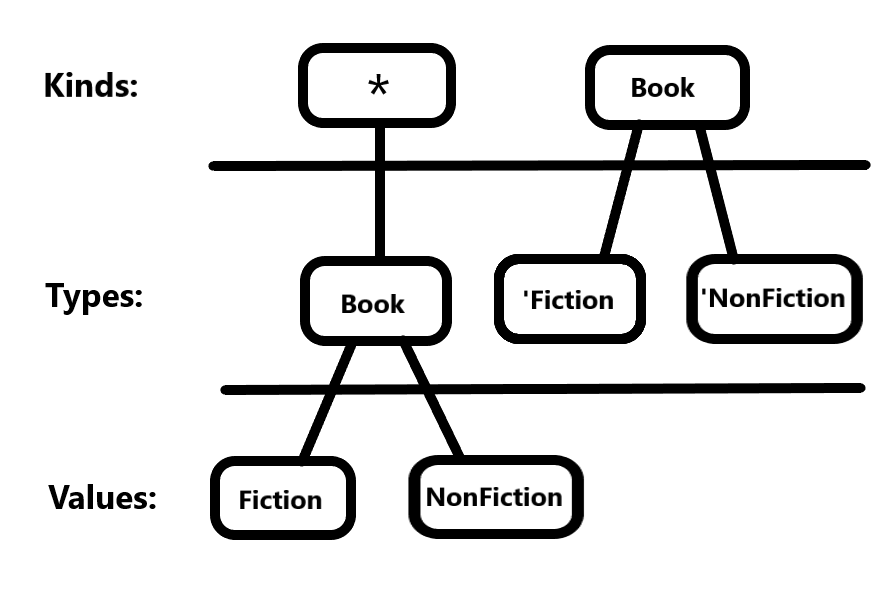
\includegraphics[height=0.6\textheight,keepaspectratio]{Promotion.png}
    \label{promotiondiagram}
\end{figure}

\end{frame}

\begin{frame}[fragile]{A Little Terminology cont.}

In Haskell, you compute on values with \emph{functions}.

\begin{lstlisting}
factorial :: Int -> Int
factorial 0 = 1
factorial x = x * factorial (x - 1)
\end{lstlisting}

\pause

But you have to use type families to compute on types:

\begin{lstlisting}
type family Factorial (x :: Nat) :: Nat where
    Factorial 0 = 1
    Factorial x = Mult x (Factorial (x - 1))
    
type family Mult (x :: Nat) (y :: Nat) :: Nat where
    Mult 0 y = 0
    Mult 1 y = y
    Mult x y = y + (Mult (x - 1) y)
\end{lstlisting}

\end{frame}

\begin{frame}[fragile]{Problems with Type Families?}

Lots of idiomatic Haskell code relies on functions being \emph{first-class}; partial application, mapping, etc.

\begin{lstlisting}
x = map (+ 2) [1,2,3]
-- = [3,4,5]
\end{lstlisting}

\pause

But type families can't be partially applied!

\begin{lstlisting}
-- Type error: type family (+) was expecting 2 arguments, got 1
type X = Map (+ 2) '[1,2,3]
\end{lstlisting}
    
\end{frame}

\begin{frame}[fragile]{Introducing First Class Families}

Thanks to Li-yao Xia, we have First Class Families!

It relies on a data type \inline{Exp}, and a type family \inline{Eval}, to create a type-level interpreter:

\begin{lstlisting}
type Exp a = a -> *
type family Eval (e :: Exp a) :: a
\end{lstlisting}

% You define a new \emph{data type} to hold the arguments, where the return types are wrapped in \inline{Exp}, and an \inline{Eval} instance to define the behaviour of the function.

\end{frame}

\begin{frame}[fragile]{Making a First Class Family}

\begin{lstlisting}
type family Not (x :: Bool) :: Bool where
    Not False = True
    Not True  = False
\end{lstlisting}

becomes:

\begin{lstlisting}
data Not :: Bool -> Exp Bool
type instance Eval (And True)  = False
type instance Eval (And False) = True
\end{lstlisting}

\end{frame}

\begin{frame}[fragile]{Type-Level Mapping}

With the below definition of \inline{Map}:

\begin{lstlisting}
data Map :: (a -> Exp b) -> f a -> Exp (f b)
type instance Eval (Map f '[])       = '[]
type instance Eval (Map f (x ': xs)) = Eval (f x) ': Eval (Map f xs)
\end{lstlisting}

And a definition of a type-level \inline{(+)}:

\begin{lstlisting}
data (:+) :: Nat -> Nat -> Exp Nat
type instance Eval (Z     :+ y) = y
type instance Eval ((S x) :+ y) = S (x :+ y)
\end{lstlisting}

We can now map over a type-level list:

\begin{lstlisting}
Eval (Map (:+ 2) '[1,2,3])
-- = '[3,4,5]
\end{lstlisting}

\end{frame}

\begin{frame}[fragile]{Representing Movement}

% In Chesskell, we represent movement with a single First Class Family that performs the given movement on a \inline{BoardDecorator}:

Each turn of movement is expressed as a single First Class Family:

\begin{lstlisting}
data Move :: Position -> Position -> BoardDecorator -> Exp BoardDecorator
\end{lstlisting}

\pause

Thanks to First Class Families, we can extend this with rule-checking naturally; using a type-level version of the function composition operator, \inline{(.)}:

\begin{lstlisting}
PostMoveCheck2 . PostMoveCheck1 . Move fromPos toPos . PreMoveCheck2 . PreMoveCheck1
\end{lstlisting}

\end{frame}

\begin{frame}[fragile]{The Board type}

To avoid repeated length checks, we use \emph{length-indexed vectors} with a type-level implementation of Peano natural numbers:

\begin{lstlisting}
data Vec (n :: Nat) (a :: Type) where
    VEnd   :: Vec Z a
    (:->)  :: a -> Vec n a -> Vec (S n) a
\end{lstlisting}

Since a Chess board is always an 8x8 grid, we use vectors of vectors:

\begin{lstlisting}
type Eight = (S (S (S (S (S (S (S (S Z))))))))
type Row   = Vec Eight (Maybe Piece)
type Board = Vec Eight Row
\end{lstlisting}

In the codebase, we use a wrapper data structure (named \inline{BoardDecorator}) to hold additional useful information.

\end{frame}

\begin{frame}[fragile]{Using the Type-Level Model}

To interact with this type level model, the output of each \inline{Move} call is piped to the next one:

\begin{lstlisting}
x = Move a1 a2 StartBoard
y = Move e3 e4 x
z = -- ...
\end{lstlisting}

\end{frame}

\begin{frame}[fragile]{Using the Type-Level Model cont.}

Below is a simplified representation of what happens for the game: \inline{chess pawn a1 to a2 king e2 to e1 end}

\begin{lstlisting}
(MoveWithCheck King e2 e1 . MoveWithCheck Pawn a1 a2) StartBoard
\end{lstlisting}

\end{frame}

% \begin{frame}[fragile]{Interacting with Type-Level model at the value level}

% The core idea is wrapping the \inline{BoardDecorator} type in a \inline{Proxy}, so that it can be passed around within a value by functions:

% \begin{lstlisting}
% data Proxy a = Proxy

% edslMove :: SPosition from
%          -> SPosition to
%          -> Proxy (b :: BoardDecorator)
%          -> Proxy (Eval (Move from to b))
% edslMove (x :: SPosition from) (y :: SPosition to) (z :: Proxy (b :: BoardDecorator))
%     = Proxy @(Eval (Move from to b))
% \end{lstlisting}

% But this would still look similar to Haskell syntax; we need a new approach.

% \end{frame}

\begin{frame}[fragile]{Creating the EDSL}

Ideally, the EDSL should look like existing chess notation:

\begin{verbatim}
1. e4 e5 2. Nf3 Nc6 3. Bb5 a6
\end{verbatim}


% Inspired by the Flat Builders pattern laid out in Mezzo.
Can achieve using Continuation Passing Style, inspired by Dima Szamozvancev's Flat Builders work (\cite{mezzo}).

\end{frame}

\begin{frame}[fragile]{Chess Continuations}

We define some important continuations: \pause \inline{chess}, \pause \inline{end}, \pause and piece continuations.

% We define a continuation for beginning the stream (named \inline{chess}), another for ending it (\inline{end}), and a series of piece continuations that move a piece of that type; \inline{king}, \inline{queen}, etc.

\pause

All of the above continuations can be chained together like so:

\begin{lstlisting}
game = chess pawn a1 to a2 bishop e4 to d5 end
\end{lstlisting}

\end{frame}

\begin{frame}[fragile]{A Longer Example}

Below is a short game, ending in checkmate by White:

\begin{figure}[h]
    \centering
    \newgame
    \scalebox{0.55}{\showboard}
    \quad
    \hidemoves{1. e4 f5 2. Qf3 g5 3. Qh5}
    \scalebox{0.55}{\showboard}
    \label{threemovecheckmate}
\end{figure}

\pause

\begin{lstlisting}
game = chess
    pawn e2 to e4
    pawn f7 to f5
    queen d1 to f3
    pawn g7 to g5
    queen f3 to h5
end
\end{lstlisting}

\end{frame}

\begin{frame}[fragile]{A Longer Example}

What about a piece trying to move after Checkmate, when the game ends?

\begin{overprint}

\onslide<1>\begin{lstlisting}
game = chess
    pawn e2 to e4
    pawn f7 to f5
    queen d1 to f3
    pawn g7 to g5
    queen f3 to h5
    pawn g5 to g4
end
\end{lstlisting}

\onslide<2>\begin{lstlisting}
-- Below results in the following type error:
    -- * The Black King is in check after a Black move. This is not allowed.
    -- * When checking the inferred type
    --     game :: Data.Proxy.Proxy (TypeError ...)
game = chess
    pawn e2 to e4
    pawn f7 to f5
    queen d1 to f3
    pawn g7 to g5
    queen f3 to h5
    pawn g5 to g4
end
\end{lstlisting}

\end{overprint}

\end{frame}

\begin{frame}[fragile]{A Longer Example cont.}

What about if the White Queen tries to move through another piece, mid-game?

\begin{overprint}

\onslide<1>\begin{lstlisting}
game = chess
    pawn e2 to e4
    pawn f7 to f5
    queen d1 to d3  -- Invalid move
    pawn g7 to g5
    queen f3 to h5
end
\end{lstlisting}

\onslide<2>\begin{lstlisting}
-- Below results in the following type error:
    -- * There is no valid move from D1 to D3.
    -- The Queen at D1 can move to: E2, F3, G4, H5, ...
    -- * When checking the inferred type
    -- game :: Data.Proxy.Proxy (...)
game = chess
    pawn e2 to e4
    pawn f7 to f5
    queen d1 to d3  -- Invalid move
    pawn g7 to g5
    queen f3 to h5
end
\end{lstlisting}

\end{overprint}

\end{frame}

\begin{frame}[fragile]{A Longer Short Example}

We also developed a shorthand syntax! 

The below game:

\begin{lstlisting}
game = chess
    pawn e2 to e4
    pawn f7 to f5
    queen d1 to f3
    pawn g7 to g5
    queen f3 to h5
end
\end{lstlisting}

becomes:

\begin{lstlisting}
game = chess
    p e4 p f5
    q f3 p g5
    q h5
end
\end{lstlisting}

\end{frame}

\begin{frame}[standout]

Demo
    
\end{frame}

\begin{frame}{Testing Overview}

Combination of:

\begin{itemize}
    \item Unit testing with assertions, based on whether a code snippet compiles or fails to compile;
    \item Unit tests of custom-made board scenarios, to test out specific behaviour;
    \item EDSL tests of custom board scenarios, for the same purpose;
    \item EDSL testing with famous Chess games, written out in Chesskell notation.
\end{itemize}
    
\end{frame}

\begin{frame}[fragile]{Unit Testing}

Unit tests rely on two main assertions; \inline{shouldTypecheck}, and \inline{shouldNotTypecheck}, which succeed or fail based on whether a specific code snippet fails with a type error or not.

We created unit tests for individual type families, to determine if they have the behaviour they should:

\begin{lstlisting}
oppositeTeamTest1 :: White :~: Eval (OppositeTeam Black)
oppositeTeamTest1 = Refl

-- ...

it "1: OppositeTeam Black = White" $
    shouldTypecheck oppositeTeamTest1
\end{lstlisting}

(Note that a value with type \inline{x :~: y} will only compile if \inline{x} and \inline{y} can be unified.)
    
\end{frame}

\begin{frame}[fragile]{Unit Testing cont.}

We also created unit tests for every FIDE Law of Chess that could be tested in this manner:

\begin{lstlisting}
whiteBishopCannotTakeOwnTeam :: Proxy (a :: BoardDecorator)
whiteBishopCannotTakeOwnTeam = Proxy @(Eval (Move (At C Nat1) (At D Nat2) WhiteStartDec))

-- ...

it "1: A White Bishop cannot take a piece on the same team" $
    shouldNotTypecheck whiteBishopCannotTakeOwnTeam
\end{lstlisting}
    
\end{frame}

\begin{frame}[fragile]{Scenario Testing}
    
We created custom Chess test boards, paired with unit tests, to model specific behaviour: % For example, we created the following board and test, whereby the Black King can castle left, but not right:

\begin{figure}[h]
    \centering
    \fenboard{8/5Q2/8/8/8/8/8/r3k2r b - - 0 1}
    \scalebox{0.55}{\showboard}
    \label{blackcastleleft}
\end{figure}

\begin{lstlisting}
blackCanCastleLeft :: '(True, False) :~: CanCastle Black BlackCastleLeftDec
blackCanCastleLeft = Refl
-- ...
shouldTypecheck blackCanCastleLeft
\end{lstlisting}

\end{frame}

\begin{frame}[fragile]{EDSL Scenario}

The EDSL was similarly tested with scenarios, to ensure that rule-breaking moves did not compile:

\begin{overprint}
    
\onslide<1>\begin{lstlisting}
didntPromoteBlack = create
        put _Wh _P at h7
        put _Bl _P at a2
    startMoves
        pawn h7 promoteTo _B h8
        pawn a2 to a1
    end
\end{lstlisting}

\onslide<2>\begin{lstlisting}
-- Below fails with the following type error:
    -- * Promotion should have occurred at: a1. Pawns must be promoted when they reach the opposite end of the board.
    -- * When checking the inferred type:
    --     didntPromoteBlack :: Data.Proxy.Proxy (TypeError ...)
didntPromoteBlack = create
        put _Wh _P at h7
        put _Bl _P at a2
    startMoves
        pawn h7 promoteTo _B h8
        pawn a2 to a1
    end
\end{lstlisting}

\end{overprint}
    
\end{frame}

\begin{frame}[fragile]{EDSL Game Testing}
    
Testing for EDSL correctness primarily consisted of writing out the first few moves of some famous game, and then making variations with errors:

\begin{overprint}

\onslide<1>\begin{lstlisting}
loopVsGandalf = chess
        p e4 p c5
        n f3 p d6
        p d4 p d4
        n d4 n f6
        n c3 p a6
    end
\end{lstlisting}

\onslide<2>\begin{lstlisting}
loopVsGandalfError = chess
        p e4 p c5
        n f3 p d6
        p d4 p d4
        n d4 n f6
        n c3 p a7
    end
\end{lstlisting}

\onslide<3>\begin{lstlisting}
loopVsGandalfError = chess
        p e4 p c5
        n f3 p d6
        p d4 p d4
        n d4 n f6
        n c3 p a7  -- Pawn moves to same place!
    end
\end{lstlisting}

\end{overprint}

\end{frame}

\begin{frame}{Compile-time and memory issues}

Compile-time and memory issues came up time and again throughout development; putting a hard limit on the length of Chesskell games.

With some games, GHC will run out of memory (\textgreater 25GB) and crash.

Through testing, it seems the upper limit is \textbf{12 moves maximum}; while all 6-move games tested have compiled, most 8- and 10-move games do as well.
    
\end{frame}

\begin{frame}[fragile]{Compile-time and memory issues cont.}

In fact, we discovered a difference in behaviour between type applications (\cite{typeapplication}) and type signatures:

\begin{lstlisting}
-- Compiles, but would hang
chess :: Spec (Proxy StartDec)
chess cont = cont (Proxy @StartDec)

-- Would fail to compile
chess :: Spec (Proxy StartDec)
chess cont = cont (Proxy :: Proxy StartDec)
\end{lstlisting}

\pause

So we filed a GHC bug report: \url{https://gitlab.haskell.org/ghc/ghc/-/issues/18902}
    
\end{frame}

\begin{frame}{Project Management}

The project was managed successfully, making use of:

\begin{itemize}
    \item Spiral methodology;
    \item Git and GitHub for version control;
    \item Weekly supervisor meetings;
    \item A Trello board to track upcoming tasks and completed features (Figure \ref{trello}); 
    \item Extensive unit and integration testing.
\end{itemize}

\pause

The implementation of Chesskell was feature-complete by the 4th of December; since then, work has gone into optimisation, testing, and write-ups.

% Ultimately, since there is no customer, an agile approach would have been a waste-so we used the \emph{spiral} methodology, moving from planning to implementation to internal testing, and repeating until done.

\end{frame}

\begin{frame}{Project Management cont.}
\begin{figure}
    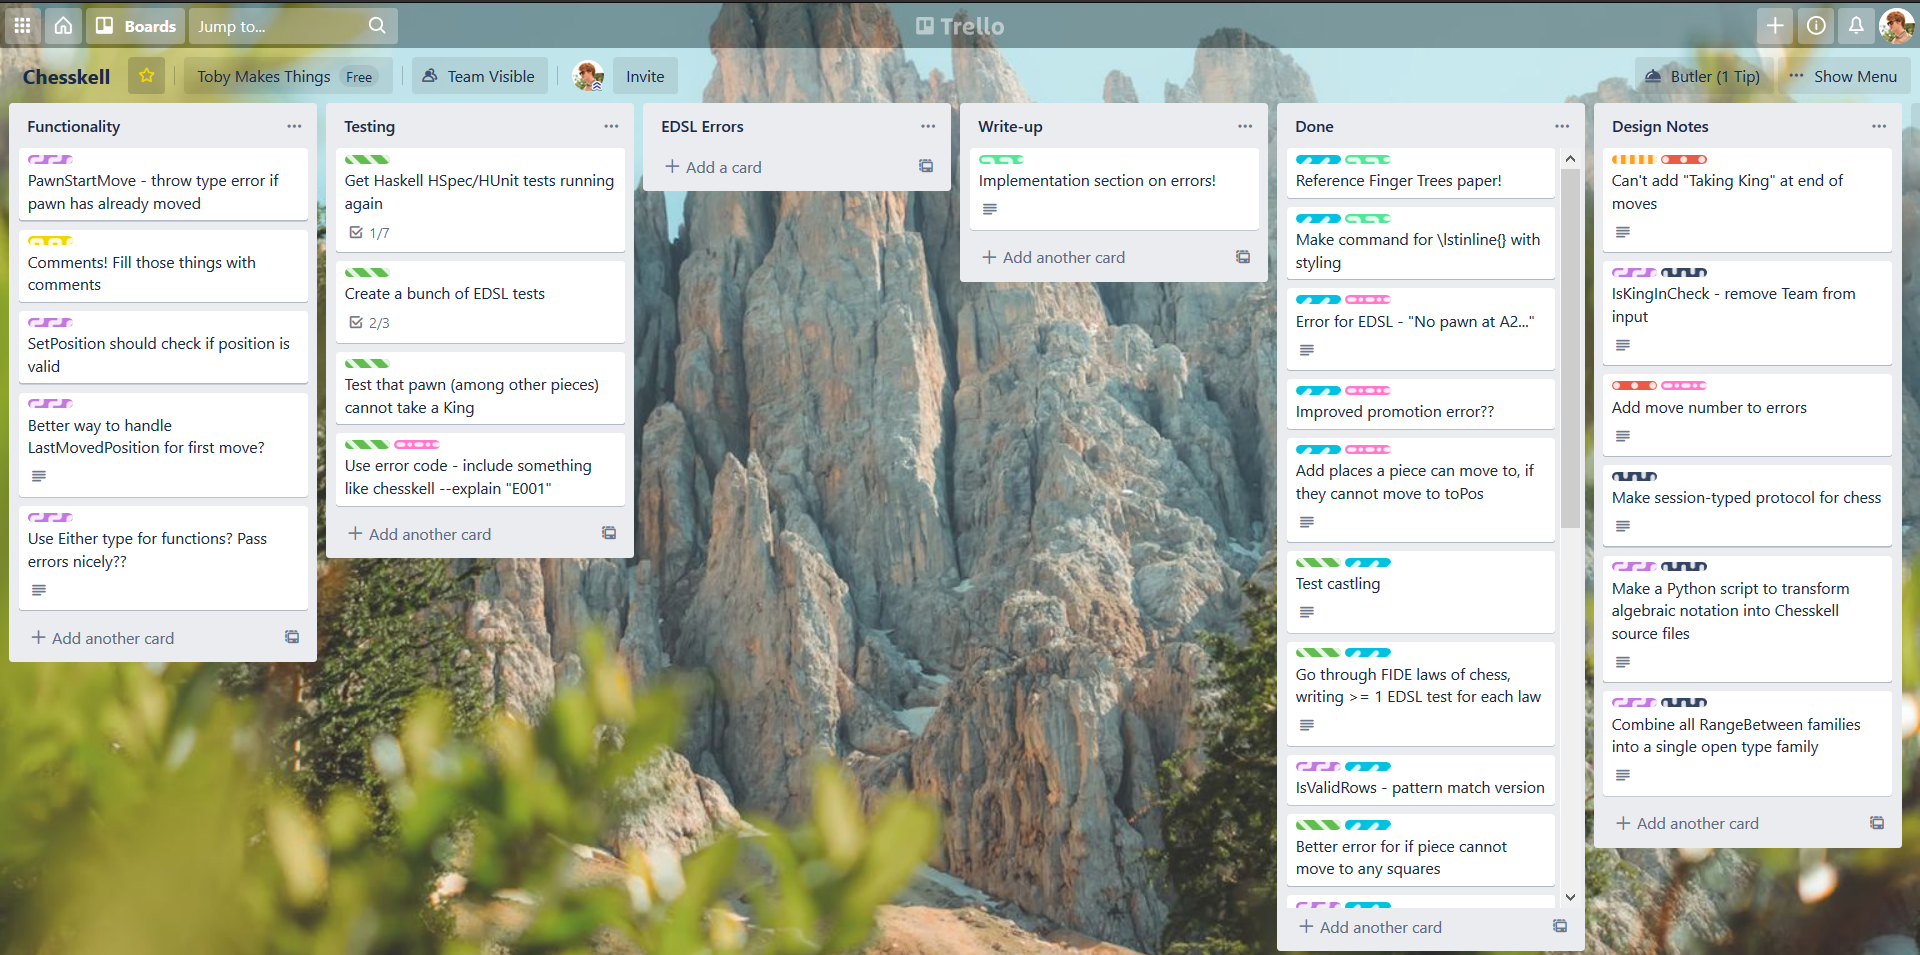
\includegraphics[width=\linewidth]{trello.png}
    \caption{The Trello board used to track development.}
    \label{trello}
\end{figure}
\end{frame}

\begin{frame}{Further Work}

There is room to expand Chesskell:

\pause

\begin{itemize}
    \item<2-> A session-typed version of Chesskell;
    \item<3-> Further optimisations to try and increase the move limit;
    \item<4-> An automated tool to transform from Algebraic Notation into Chesskell notation.
\end{itemize}
    
\end{frame}

\begin{frame}{Conclusions}

We have created:

\pause

\begin{itemize}
    \item<2-> A full type-level model of Chess, which enforces all rules in the FIDE 2018 Laws of Chess;
    \item<3-> An EDSL for describing Chess games and creating custom chess boards, which uses the type-level model for rule-checking;
    \item<4-> At the end of next week, we will submit a Haskell Symposium paper about the development of Chesskell, including our findings on compile-time and memory usage issues.
\end{itemize}

\begin{overprint}
\onslide<5>Furthermore, Chesskell is unique and has never been done before. Though there is room for further work and improvement, Chesskell is a success!
\end{overprint}

    
\end{frame}

\begin{frame}[standout]

Q\&A
    
\end{frame}

\begin{frame}[allowframebreaks]{References}

\printbibliography
    
\end{frame}

\end{document}
